\documentclass{beamer}
\usepackage[utf8]{inputenc}
%%\usetheme{Kalgan}
\setbeamercovered{highly dynamic}
\setbeamersize{text margin left=5pt}
\usepackage{listings}
\lstset{
  language=Python,
  basicstyle=\ttfamily\scriptsize,
  breaklines=false
}
\usepackage{graphicx}
\graphicspath{{../res/}}
\DeclareGraphicsExtensions{.pdf,.jpg,.png}
\usepackage{animate}

\usepackage[czech,english]{babel}
\usepackage[cmex10]{amsmath}
\usepackage{amsfonts}
\usepackage{amssymb}
\usepackage{amsthm}
\usepackage{thm-restate}
\usepackage{gensymb}
\usepackage[linesnumbered,ruled,noend]{algorithm2e}
\usepackage[utf8]{inputenc}
\usepackage[pdftex]{graphicx}
\usepackage{subfig}
\usepackage{mathtools}
\usepackage{tikz}
\usepackage{listings}
\usepackage{verbatim}
\usepackage{float}
\usepackage{hyperref}
\usepackage{cleveref}
\usepackage{setspace}
\usepackage{xpatch}

\newcommand{\andspc}{\;\;\land\;\;}
\definecolor{myblue}{RGB}{80,80,160}
\definecolor{mygreen}{RGB}{80,160,80}

\DeclarePairedDelimiter{\ceil}{\lceil}{\rceil}
\DeclarePairedDelimiter{\floor}{\lfloor}{\rfloor}

\renewcommand{\vec}[1]{\ensuremath{\mathbf{#1}}}
\renewcommand{\l}{\left}
\renewcommand{\r}{\right}

\newcommand{\avec}[1]{\ensuremath{\tilde{\mathbf{#1}}}}
\newcommand{\ds}[1]{\ensuremath{\,\,#1\,\,}}
\newcommand{\dsand}{\ds{\land}}
\newcommand{\textds}[1]{\ds{\ds{\text{#1}}}}
\newcommand{\comma}{\ensuremath{\ds{\ds{\ds{,}}}}}
\newcommand{\toprove}{\ensuremath{\ds{\vdash}}}
\newcommand{\imply}{\ensuremath{\,\,\,\,\Rightarrow\,\,\,\,}}
\newcommand{\fromto}{\ensuremath{\rightarrow}}
\newcommand{\bigO}[1]{\ensuremath{\operatorname{O}\left(#1\right)}}
\newcommand{\bigW}[1]{\ensuremath{\operatorname{\Omega}\left(#1\right)}}
\newcommand{\bigT}[1]{\ensuremath{\operatorname{\Theta}\left(#1\right)}}
\newcommand{\R}[1]{\ensuremath{\,\mathbb{R}^{#1}\,}}
\newcommand{\trans}[1]{\ensuremath{\,{#1}^{T}\,}}
\newcommand{\func}[1]{\ensuremath{\operatorname{#1}}}
\newcommand{\inv}[1]{\ensuremath{{#1}^{-1}}}
\newcommand{\apos}[1]{\textsc{\char13}#1}
\newcommand{\prim}[1]{{#1}^\apos{}}
\newcommand{\ortc}[1]{\ensuremath{{#1}^{\bot}}}
\newcommand{\C}[1]{\ensuremath{\func{C}(#1)}}
\newcommand{\N}[1]{\ensuremath{\func{N}(#1)}}
\renewcommand{\dim}[1]{\ensuremath{\func{dim}(#1)}}
\newcommand{\abs}[1]{\ensuremath{\left\lvert #1 \right\vert}}
\newcommand{\norm}[1]{\ensuremath{\left\lVert #1 \right\rVert}}
\newcommand{\Rehurek}{\v{R}eh{u}\v{r}ek }

\newcommand\xqed{%
  \leavevmode\unskip\penalty9999 \hbox{}\nobreak\hfill
  \quad\hbox{$\triangle$}}

\newcommand{\suchthat}{%
  \ensuremath{\mathrel{\,\,\ooalign{$\ni$\cr\kern-1pt$-$\kern-6.5pt$-$}}\,\,}}



\title{Parallel and Distributed Computing: \\Singular Value Decomposition in the
context of massive online Latent Semantic Indexing}
\author{Bahena, Zavaleta}%
\institute{CINVESTAV - ORACLE}
\date{August, 2015}

\begin{document}
	\begin{frame}[plain]
	  \titlepage
	\end{frame}
  %%%%%%%%%%%%%%%%%%%%%%%%%%%%%%%%%%%%%%%%%%%%%%%%%%%%%%%%%%%%%%%%%%%%%%%%%%%%%%%%
\begin{frame} [plain]
\frametitle{SVD Decomposition}
\begin{block}{}
$A = U \Sigma V^{T}$
\begin{itemize}
  \item $U$ and $V$ are orthogonal matrices
  \item $\Sigma$ is a diagonal matrix that contain the \textit{singular values} $\sigma_i$ of
A; $\sigma_1 \geq \sigma_2 \geq ... \geq \sigma_n \geq 0$
\end{itemize}
\end{block}
\begin{block}{}
In the 20th century, focus was on obtaining efficient algorithms for SVD
computation
\begin{itemize}
  \item Several implementations of SVD solvers
  \begin{itemize}
    \item SVDPACK(C)
    \item SVDLIBC
    \item LAPACK
    \item ...
  \end{itemize}
  \item Gensim contains the SVD solver that best matches our problem (as far as we could investigate)
\end{itemize}
\end{block}
\end{frame}
%%%%%%%%%%%%%%%%%%%%%%%%%%%%%%%%%%%%%%%%%%%%%%%%%%%%%%%%%%%%%%%%%%%%%%%%%%%%%%%%



  \begin{frame}[plain]
  \frametitle{Latent Semantic Indexing}
  \begin{block}{}
  Documents are encoded using the Vector Space Model 
  \begin{itemize}
    \item A matrix $A$ of size $m \times n$
    \item $m$ indexed terms
    \item $n$ documents
  \end{itemize}
  \end{block} 

  \begin{block}{}
    The VSM can not handle ambiguity:
    \begin{itemize}
    \item Synonymity
    \item Polysemy
    \end{itemize}
  \end{block} 
\end{frame}
%%%%%%%%%%%%%%%%%%%%%%%%%%%%%%%%%%%%%%%%%%%%%%%%%%%%%%%%%%%%%%%%%%%%%%%%%
	\begin{frame}[plain]
	 	\frametitle{Latent Semantic Indexing}
		\begin{block}{}
\begin{table}[]
\centering
\begin{tabular}{|l|l|l|l|l|l|l|}
\hline
             & {\bf d1} & {\bf d2} & {\bf d3} & {\bf d4} & {\bf d5} & {\bf d6} \\ \hline
{\bf ship}   & 1        & 0        & 1        & 0        & 0        & 0        \\ \hline
{\bf boat}   & 0        & 1        & 0        & 0        & 0        & 0        \\ \hline
{\bf ocean}  & 1        & 1        & 0        & 0        & 0        & 0        \\ \hline
{\bf voyage} & 1        & 0        & 0        & 1        & 1        & 0        \\ \hline
{\bf trip}   & 0        & 0        & 0        & 1        & 0        & 1        \\ \hline
\end{tabular}
\caption{Terms-Documents matrix }
\label{table:example00}
\end{table}
		\end{block} 
	\end{frame}
%%%%%%%%%%%%%%%%%%%%%%%%%%%%%%%%%%%%%%%%%%%%%%%%%%%%%%%%%%%%%%%%%%%%%%%%%
\begin{frame}[plain]
  \frametitle{Latent Semantic Indexing and the Truncated SVD}
  \begin{block}{}
  According to Deerwester et al. there is a latent space
where documents and indexed terms are expresed with $r$ features.
  \begin{itemize}
    \item $A = U \Sigma V^{T}$
    \item $U$ is the matrix of terms
    \item $V$ is the matrix of documents
    \item $\Sigma$ contains $r$ singular values
  \end{itemize}
  \end{block}

  \begin{block}{}
  The smallest singular values are actually noise and we can
get rid of them
  \begin{itemize}
    \item By doing so we get $A_k = U_k \Sigma_k V_k^{T}$
    \item This step is justified by Eckart-Young-Mirsky theorem 
\begin{equation} 
\min_{\{Z|rank(Z)=k\}} \|A-Z\|_{2} = \|A-A_{k}\|_{2} = \sigma_{k+1}
\end{equation}
  \end{itemize}
  \end{block}
\end{frame}
%%%%%%%%%%%%%%%%%%%%%%%%%%%%%%%%%%%%%%%%%%%%%%%%%%%%%%%%%%%%%%%%%%%%%%%%%
\begin{frame}[plain]
  \frametitle{Latent Semantic Indexing and the Truncated SVD}
  \begin{block}{}
  1) In this space, to compare two terms:
\begin{equation}
A_{k}A_{k}^{T} = U_k \Sigma_k^{2} U_k^{T}
\end{equation}
  \end{block}

  \begin{block}{}
  2) To compare two documents:
\begin{equation}
A_{k}^{T} A_{k} = V_k \Sigma_k^{2} V_k^{T}
\end{equation}
  \end{block}

  \begin{block}{}
  3) The association between a term $i$ and a document $j$ is given by the value in
position $ij$ in matrix $A_k$
  \end{block}
\end{frame}

  %%%%%%%%%%%%%%%%%%%%%%%%%%%%%%%%%%%%%%%%%%
	\begin{frame}[plain]
	 	\frametitle{LSI: A quick example}
\begin{equation}
 U =
\begin{pmatrix}
 -0.45 & -0.30 & 0.57 & 0.58 & 0.25 \\
 -0.13 & -0.33 & -0.59 & 0 & 0.73 \\
 -0.48 & -0.51 & -0.37 & 0 & -0.61 \\
 -0.70 & 0.35 & 0.15 & -0.58 & 0.16\\
 -0.26 & 0.65 & -0.41 & 0.58 & -0.09 \end{pmatrix}
\end{equation}
\begin{equation}
 \Sigma =
\begin{pmatrix}
 2.16 & 0 & 0 & 0 & 0\\
 0 & 1.59 & 0 & 0 & 0\\
 0 & 0 & 1.28 & 0 & 0\\
 0 & 0 & 0 & 1.00 & 0\\
 0 & 0 & 0 & 0 & 0.39 \end{pmatrix}
\end{equation}
\begin{equation}
  V^{T} = 
\begin{pmatrix}
 -0.75 & -0.28 & -0.20 & -0.45 & -0.33 & -0.12\\
 -0.29 & -0.53 & -0.19 &  0.63 &  0.22 &  0.41\\
  0.28 & -0.75 &  0.45 & -0.20 &  0.12 & -0.33\\
  0    &  0    &  0.58 &  0    & -0.58 &  0.58\\
 -0.53 &  0.29 &  0.63 &  0.19 &  0.41 & -0.22 \end{pmatrix}
\end{equation}
	\end{frame}
%%%%%%%%%%%%%%%%%%%%%%%%%%%%%%%%%%%%%%%%%%
\begin{frame}[plain]
\frametitle{LSI: A quick example}
\begin{equation}
 \Sigma_{2} =
\begin{pmatrix}
 2.16 & 0.00 \\
 0.00 & 1.59 \end{pmatrix}
\end{equation}
\\
\begin{equation}
A_{2} = \begin{pmatrix}
    1.0199 &   0.0060 &   1.0112 &   0.0095 &   0.0069 &  -0.0047 \\
    0.0004 &   1.0057 &  -0.0046 &   0.0009 &   0.0033 &   0.0052 \\
    1.0062 &   1.0063 &  -0.0016 &   0.0052 &   0.0094 &   0.0006 \\
    0.9933 &   0.0025 &  -0.0140 &   1.0045 &   1.0064 &  -0.0039 \\
   -0.0069 &  -0.0071 &  -0.0059 &   1.0021 &  -0.0011 &   1.0084 \end{pmatrix}
\end{equation}
\\
\begin{equation}
\|A - A_{k}\|_{2} = 1.28
\end{equation}
\\
\begin{equation}
\Sigma_{2} V_{2}^{T} = \begin{pmatrix}
 -1.62 & -0.60 & -0.44 & -0.97 & -0.70 & -0.26\\
 -0.46 & -0.84 & -0.30 &  1.00 &  0.35 &  0.65 \end{pmatrix} 
\end{equation}
\end{frame}
%%%%%%%%%%%%%%%%%%%%%%%%%%%%%%%%%%%%%%%%%%
\begin{frame}[plain]
\frametitle{LSI: A quick example}
\begin{equation}
q = \begin{pmatrix}0\\1\\0\\0\\0\end{pmatrix}
\end{equation}\
\\
\begin{equation}
q_{k} = \begin{pmatrix}-0.06\\-0.21\end{pmatrix}
\end{equation}
\end{frame}
%%%%%%%%%%%%%%%%%%%%%%%%%%%%%%%%%%%%%%%%%%
\begin{frame}[plain]
\frametitle{LSI: A quick example}
\begin{center}
  \begin{figure}[H]
    \centering
    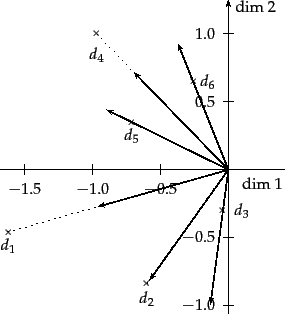
\includegraphics[width=5cm]{space.png}
    \label{fig:spaces}
  \end{figure}
\end{center}
\end{frame}


  \begin{frame}[plain]
  \frametitle{How did we come up with this idea?}
  \begin{block}{}
    Looking for ideas for a Msc. Thesis
    \begin{itemize}
      \item Possibly apporting something to Oracle :)
    	\item Oracle bought \textit{Collaborative Intellect Inc.} in 2012
    \begin{itemize}
      \item Analytics engine that processes conversations from Social Networks
      	\item Companies using this product can know if user's posts in
          Social Networks are associated with certain topics they
          define (which can be their products, services, etc).
      \item Tens of Millions of conversations in a day!
      \item Social Networks produce Hundreds of Millions!
      \item Requires LSI!
    \end{itemize}
     \end{itemize}
  \end{block} 
\end{frame}
%%%%%%%%%%%%%%%%%%%%%%%%%%%%%%%%%%%%%%%%%%%%%%%%%%%%%%%%%%%%%%%%%%%%%%%%%%%%%
\begin{frame}[plain]
  \frametitle{How did we come up with this idea?}
\begin{center}
  \begin{figure}[H]
    \centering
    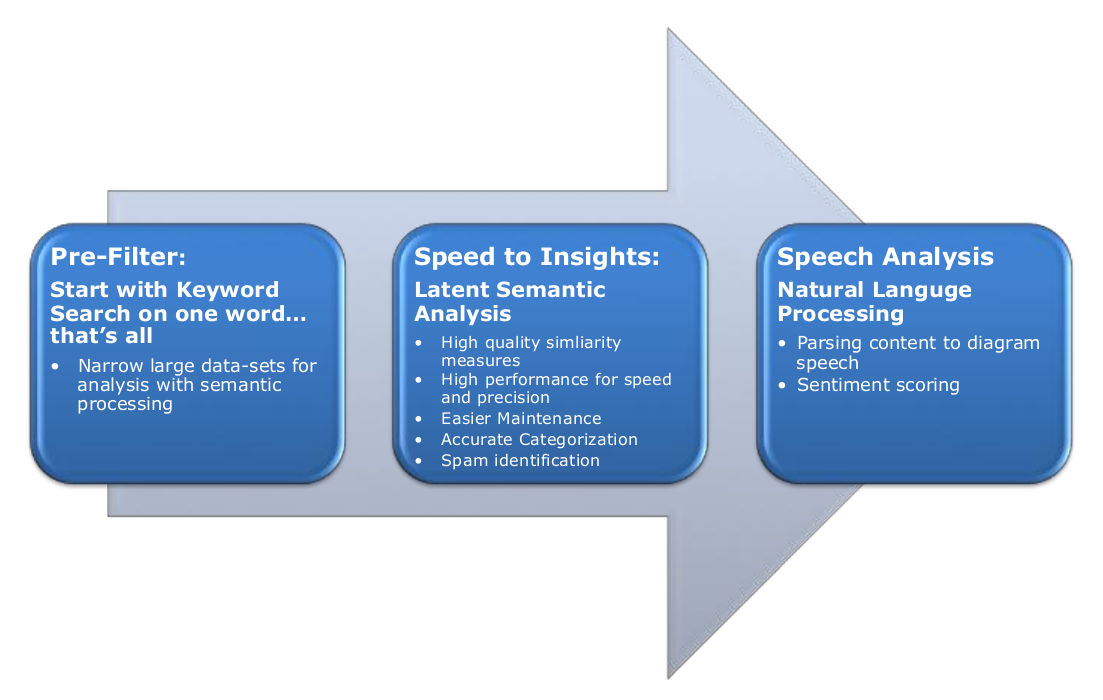
\includegraphics[width=10cm]{oracle.png}
  \end{figure}
\end{center}
\end{frame}
%%%%%%%%%%%%%%%%%%%%%%%%%%%%%%%%%%%%%%%%%%%%%%%%%%%%%%%%%%%%%%%%%%%%%%%%%%%%%
\begin{frame}[plain]
  \frametitle{Statement of the Problem}
  \begin{block}{}
  \textit{Given the fact that modern LSI applications require end to end
processing of hundreds of millions of documents every day, in a streamed
updatable fashion, how can the particular SVD step be optimized through parallel
or distributed computing?}
  \end{block} 
\end{frame}

  \begin{frame}[plain]
	\frametitle{What does $A = U \Sigma \trans{V}$ mean?}
	\begin{block}{Geometric interpretation}
    \begin{center}
      \begin{figure}[H]
        \centering
        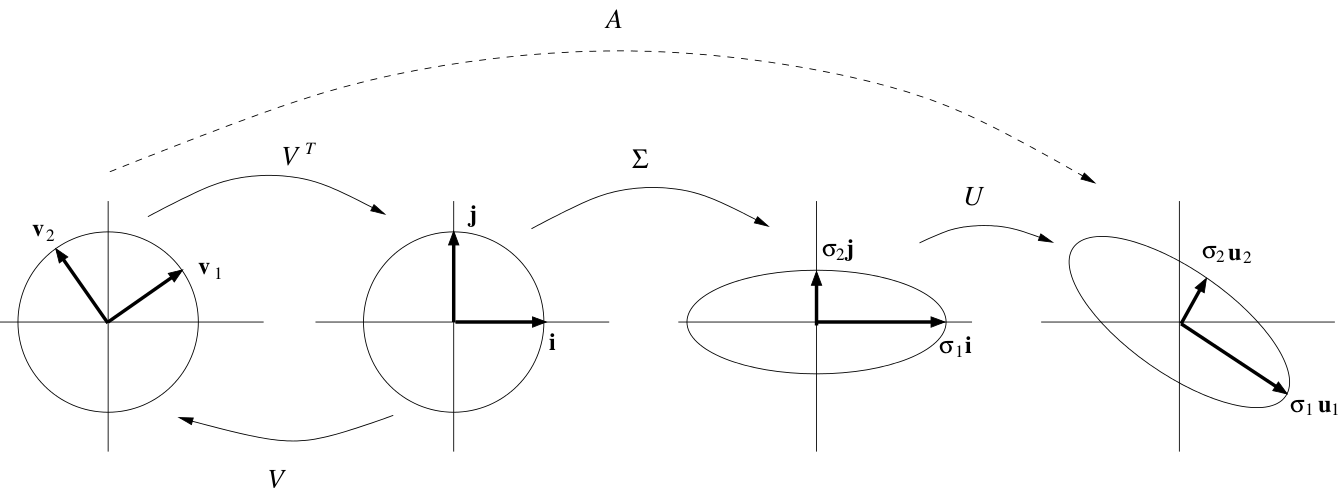
\includegraphics[width=10cm]{svd-geo-diag}
      \end{figure}
    \end{center}
	\end{block} 
\end{frame}

%%  \begin{frame}[plain]
	\frametitle{Why SVD is possible? Geometrical insight}
	\begin{block}{Is all about orthogonality}
    $A = U \Sigma \trans{V} \ds{\implies} A\vec{v_i} = \sigma_i
    \vec{u_i} \suchthat i=1\dots\func{rank}(A)$
	\end{block}   
	\begin{block}{What is special about \vec{v}?}
    \begin{center}
      \begin{figure}[H]
        \centering
        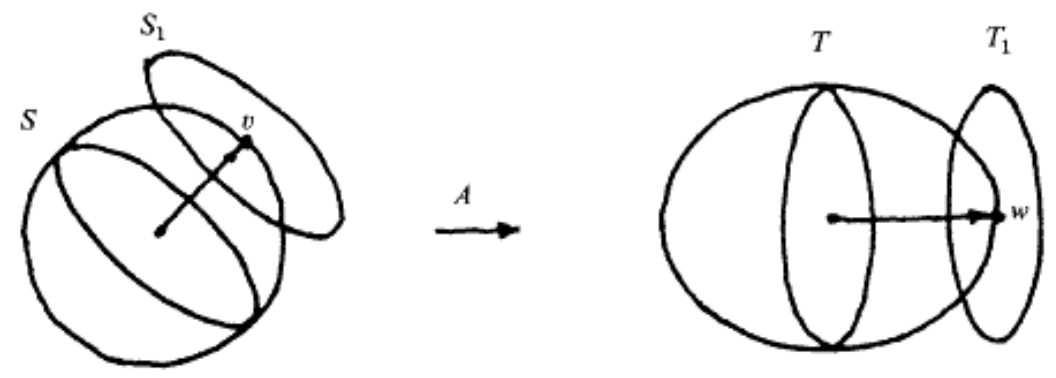
\includegraphics[width=10cm]{svd-geo-proof}
      \end{figure}
    \end{center}
	\end{block} 
	\begin{block}{Got curious?}
    Check the report, it has the full proof.
	\end{block}   
\end{frame}

  \begin{frame}[plain]
	\frametitle{SVD as an Eigenproblem}
	\begin{block}{Algebraic and Geometric Proofs}
    A whole chapter of the report, check it out!
	\end{block}   
	\begin{block}{The eigenproblem, solved for symmetric matrices}
    $B^{n \times n} = Q\,\Lambda\trans{Q}$
	\end{block}
	\begin{block}{$\trans{A}A$ is symmetric!}
    $A = U\, \Sigma \trans{V} \ds{\ds{\iff}} \trans{A}A = V\, \Sigma^2 \trans{V}$
	\end{block}   
	\begin{block}{$A\trans{A}$ is symmetric too! (used in GenSim)}
    $A = U\, \Sigma \trans{V} \ds{\ds{\iff}} A\trans{A} = U\, \Sigma^2 \trans{U}$
	\end{block}
\end{frame}

  \begin{frame}[plain]
	\frametitle{Is SVD problem well conditioned?}
	\begin{block}{A problem is well conditioned if ... }
    $x \simeq (x+\delta) \implies f(x) \simeq f(x + \delta)$
	\end{block}   
	\begin{block}{Weyl's Theorem}
    $\abs{\tilde{\sigma_i} - \sigma_i} \le \norm{E}_2 \ds{\suchthat}
    \tilde{A} = A + E$
	\end{block}
	\begin{block}{Wedin's Theorem}
    The singular vectors subproblem is not well conditioned in theory,
    but it has bounds.
	\end{block}
	\begin{block}{In practice we are fine}
    We do not need singular vectors by themselves ($\vec{v} =
    \inv{\Sigma}\trans{U}\vec{x}$).
	\end{block}
\end{frame}

  \begin{frame}[plain]
	\begin{block}{}
\begin{algorithm}[H]
  \label{alg:lasvd}
  \caption{The Single-Vector Lanczos Algorithm}
%
  \SetKwInOut{Input}{Input}
  \SetKwInOut{Output}{Output}
  \DontPrintSemicolon
%
    \Input{A matrix $A^{m \times n}$ and a truncation factor
    $k$}
%
    \Output{The $k$ singular values and its associated right singular
      vectors of $A$. Both are numeric approximations.}
%
    \BlankLine
    Use Lanczos Tridiagonalization Step to generate a family of
    $c$ symmetric tridiagonal matrices $\{ T_j \}$ for $\trans{A}A$
    ($c > k$) \;
    \BlankLine
%
    Compute the eigenvalues and eigenvectors of $T_k$ using the
    (implicit) QL Method. \;
    \BlankLine
%   
    For each computed $\lambda_i$ of $T_k$, calculate the associated
    unit eigenvector $\vec{z_i}$ such that $T_k\vec{z_i} =
    \lambda_i\vec{z_i}$. \; 
    \BlankLine
% 
    For each calculated eigenvector $\vec{z_i}$ of $T_k$, compute the Ritz
    vectors $v_i = Q_c\vec{z_i}$ as an approximation to the
    $i$-th eigenvector of $\trans{A}A$. Note that the matrix $Q_c$ is
    a side product of the first step. \; 
    \BlankLine
%
    return $(\{\sqrt{\lambda_1},\sqrt{\lambda_2},\cdots,
    \sqrt{\lambda_k}\},
            \{\vec{v_1},\vec{v_2},\cdots,\vec{v_k}\})$
%
\end{algorithm}
	\end{block} 
\end{frame}

  \begin{frame}[plain]
	\begin{block}{}
\begin{algorithm}[H]
%
  \caption{Lanczos Tridiagonalization Step (sparse,2)}
  \setstretch{1.5}
  \SetKwInOut{Input}{Input}
  \SetKwInOut{Output}{Output}
  \DontPrintSemicolon
%
    \Input{A unit vector $\vec{q_1} \in \R{n}$ and a symmetric matrix $A^{n
        \times n}$}
%
    \Output{The sequences $\{\alpha_i\}$, $\{\beta_i\}$ and matrix $Q
      = [ \vec{q_1} | \vec{q_2} | \cdots ]$ }
%
    $k \gets 0, \beta_0 \gets 1, \vec{q_0} \gets 0, r_0 \gets \vec{q_1}$ \;
    \While {$k = 0 \lor \beta_k \ne 0$}
    {
      $\vec{q_{k+1}} \gets \dfrac{\vec{r_k}}{\beta_k}$ \;
      $k \gets k + 1$ \;
      $\alpha_k \gets \trans{\vec{q_k}}A\vec{q_k}$ \;
      $\vec{r_k} \gets A\vec{q_k} - \alpha_kq_k - \beta_{k-1}\vec{q_{k-1}}$ \;
      $\beta_k \gets \norm{\vec{r_k}}_2$ \;
    }
%
    return $(\{\alpha_i\}, \{\beta_i\}, 
             Q = [ \vec{q_1} | \vec{q_2} | \cdots ])$ \;
\end{algorithm}
\hfill
	\end{block} 
\end{frame}

  \begin{frame}[plain]
	\frametitle{The $T_k$ from Lanczos Tridiagonalization Step}
	\begin{block}{}
    \[
    T_k = 
    \begin{bmatrix}
      \alpha_1 & \beta_1 & \cdots      & 0          \\
      \beta_1  & \ddots  & \ddots      & \vdots     \\
      \vdots   & \ddots  & \ddots      & \beta_{k-1} \\
      0        & \cdots  & \beta_{k-1} & \alpha_k
    \end{bmatrix}
    \]
    \hfill
	\end{block}
\end{frame}

  \begin{frame}[plain]
	\frametitle{Lanczos Algorithm Reality Check}
	\begin{block}{Is it numerically stable?}
    No, the tridiagonalization step needs to be rewritten (thanks Paige!).
	\end{block}   
	\begin{block}{Is orthogonality really guaranteed?}
    No, it is lost precisely with the converved singular vectors
    (thanks again Peige!). Selective re-orthogonalization is required
    (thanks Parlett and Simon!).
	\end{block}
	\begin{block}{What to do then?}
    Berry's implementation, LASVD/LAS2, consider all aspects above;
    including performance (parallelization). 
	\end{block}
\end{frame}

  \begin{frame}[plain]
	\frametitle{LASVD/LAS2 Profiling by Berry}
	\begin{block}{}
\begin{table}[!h]
\begin{center}
\begin{tabular}{|c|c|c|}
\hline
Routine & Library & Description \\
\hline
\hline
SPMXV & BLAS level 2 & Sparse matrix-vector mult. \\
\hline
IMTQL2 / TRED2 & EISPACK & Implicit QL Algorithm. \\
\hline
DAXPY & BLAS level 1 & $\vec{x} \gets \gamma \vec{x} + \vec{y}$ \\
\hline
DAXPY & BLAS level 1 & $\vec{x} \gets \vec{y}$ \\
\hline
DDOT & BLAS level 1 & $\vec{x} \cdot \vec{y}$ \\
\hline
\end{tabular}
\end{center}
\end{table}
\begin{table}[!h]
\begin{center}
\begin{tabular}{|c|c|c|c|c|}
\hline
& \multicolumn{2}{|c|}{Alliant FX/80} & \multicolumn{2}{|c|}{Cray-2S/4-128} \\
\hline
Routine & Speedup & \%CPU Time & Speedup & \%CPU Time \\
\hline
\hline
SPMXV & 3 & 27\% & - & 72\% \\
\hline
IMTQL2 & 4.3 & 14\% & - & 12\% \\
\hline
DAXPY & 5 & 17\% & - & - \\
\hline
DCOPY & 3.6 & 20\% & - & - \\
\hline
DDOT & 7.7 & 2\% & - & - \\
\hline
\hline
\end{tabular}
\end{center}
\end{table}
	\end{block}  
\end{frame}

  \begin{frame}[plain]
	\frametitle{SVDPACK $\implies$ SVDLIBC: lost parallelism}
	\begin{block}{}
    \begin{itemize}
      \item Berry's SVDPACK LAS2: SPMXV (BLAS?), IMTQL2 (EISPACK)
      \item Berry ports to SVDPACKC: opa/opb (user), IMTQL2 (serial!)
      \item Rohde new skin of SVDLIBC: opa/opb (serial!),
        IMTQL2 (serial!).
      \item Radim's python wrapper SPARSESVD : same all
      \item Radim's GenSim uses a serial LAS2 routine!
    \end{itemize}
	\end{block}
\end{frame}

  \begin{frame}[plain]
\begin{algorithm}[H] 
  \caption{Distributed-SVD: Distributed SVD for LSI (global)}
%
  \setstretch{1.35}
  \SetKwInOut{Input}{Input}
  \SetKwInOut{Output}{Output}
  \DontPrintSemicolon
%
    \Input{Truncation factor $k$, queue of jobs $A= [A_1, A_2, \dots ]$}
%
    \Output{Matrices $U^{m \times k}$ and $\Sigma^{k \times k}$, 
      from the SVD decomp. of $A$}
%
    \For {\textbf{all} (node $i$ in cluster)}
    {
      $B_i \gets \text{subset of the queue of jobs } [A_1,A_2,\dots]$ \;
%
      $P_i = (U_i,\Sigma_i) \gets \func{SVD-Node}(k,B_i)$ \;
    }
    $(U,\Sigma) \gets \func{Reduce}(\func{Merge-SVD},[P_1,P_2,\dots])$ \;
%
    return $(U, \Sigma)$ \;
\end{algorithm}
\end{frame}
%%%%%%%%%%%%%%%%%%%%%%%%%%%%%%%%%%%%%%%%%%%%%%%%%%%%%%%%
\begin{frame}[plain]
\begin{algorithm}[H]
  \caption{SVD-Node: Distributed SVD for LSI (node)}
%
  \setstretch{1.35}
  \SetKwInOut{Input}{Input}
  \SetKwInOut{Output}{Output}
  \DontPrintSemicolon
%
  \Input{Truncation factor $k$, queue of jobs $A_1,A_2,\dots$}
%
  \Output{Matrices $U^{m \times k}$ and $\Sigma^{k
        \times k}$, from the SVD  of $[A_1,A_2,\dots]$}
%
  $P = (U,\Sigma) \gets 0^{m \times k} 0^{k \times k}$ \;
%
  \For {each job $A_i$}
  {
    $\prim{P} = (\prim{U},\prim{\Sigma}) \gets \func{Basecase-SVD}(k,A_i)$ \;
%
    $P = (U^{m \times k},\Sigma^{k \times k}) \gets \func{Merge-SVD}(k, P, \prim{P})$ \;
  }
%
  return $(U,\Sigma)$ \;
\end{algorithm}
\end{frame}
%%%%%%%%%%%%%%%%%%%%%%%%%%%%%%%%%%%%%%%%%%%%%%%%%%%%%%%%
\begin{frame}[plain]
\begin{algorithm}[H]
  \label{alg:merge-svd}
  \caption{$\func{Merge-SVD}$: Merge of two SVD factorizations}
%
  \setstretch{1.35}
  \DontPrintSemicolon
  \SetKwInOut{Input}{Input}
  \SetKwInOut{Output}{Output}
%
  \Input{Truncation factor $k$, decay factor $\gamma$,  
    $P_1 = (U_1^{m \times k_1}, \Sigma_1^{k_1 \times k_1})$,
    $P_2 = (U_2^{m \times k_2}, \Sigma_1^{k_2 \times k_2})$}
%
  \Output{$(U^{m \times k}, \Sigma^{k \times k})$}
%
  $Z^{k_1 \times k_2} \gets \trans{U_1}U_2$ \;
%
  $\prim{U} R \xleftarrow{QR} U_2 - U_1 Z$ \;
%
  $U_R \Sigma\trans{V_R} \xleftarrow{SVD_k}
    \begin{bmatrix}
      \gamma\Sigma_1 & Z \Sigma_2 \\
      0 & R\Sigma_2
    \end{bmatrix}^{(k_1 + k_2) \times (k_1 + k_2)}$ \;
%
  $\begin{bmatrix}
      R_1^{k_1 \times k} \\
      R_2^{k2 \times k}
    \end{bmatrix} = U_R$ \;
%
  $U \gets U_1R_1 + \prim{U}R_2$ \;
%
  return $(U,\Sigma)$ \;
\end{algorithm}
\end{frame}
%%%%%%%%%%%%%%%%%%%%%%%%%%%%%%%%%%%%%%%%%%%%%%%%%%%%%%%%
\begin{frame}[plain]
\frametitle{Distributed Algorithm}
\begin{block}{}
      Complexity is according to him $O(mk^2)$
      \begin{itemize}
      \item Processed Wikipedia (3.2M documents, 100K words) in 2.5 hours in a 4 nodes cluster
      \item Using BLAS/LAPACK in the merge algorithm it took 1 hour and 41 minutes
      \item Another custom implementation of another SVD algorithm took 109
hours
      \end{itemize}
\end{block} 
\end{frame}

  \begin{frame}[plain]
\frametitle{Conclusions}
\begin{block}{}
We found that the following is still required:
\begin{itemize}
\item Enhance memory complexity study of Rehurek's algorithm
\item Need a modern sensible experiment that compares best parallel/distributed algorithms taking into account the architecture of modern computers
\begin{itemize}
\item Compare against Mahout, SLEPc, LingPipe, GraphLab, etc.
\item Use experiments similar to those that Rehurek did. 
\item Need to use much more documents and more nodes in the cluster
\item Could get benchmark matrices used by Oracle's alternative
\end{itemize}
\item For the case of Rehurek's, profiling experiments similar to those made by Berry, could help identify bottlenecks
\begin{itemize}
\item Base case SVD
\item Merge Algorithm
\end{itemize}
\end{itemize}
\end{block}
\end{frame}
%%%%%%%%%%%%%%%%%%%%%%%%%%%%%%%%%%%%%%
\begin{frame}[plain]
\frametitle{Conclusions}
\begin{block}{}
\begin{itemize}
\item Need to research whether Rehurek's merge algorithm is optimal or not
\item Need to try other merge alternatives
\item Need an experiment with different implementations of the base case SVD solver
\begin{itemize}
\item Could try parallel versions of SVDLIBC (BLAS/LAPACK)
\end{itemize}
\end{itemize}
\end{block}
\end{frame}

\end{document}
